\documentclass[a4paper]{article}
\usepackage{amsmath}
\usepackage{listings}
\usepackage{hyperref}
\usepackage{cite}
% pgfplot setting
\usepackage{pgfplots}
\pgfplotsset{width=7cm,compat=1.8}
\pgfplotsset{%
  colormap={whitered}{color(0cm)=(white);
  color(1cm)=(orange!75!red)}
}
% references
\bibliographystyle{plain}
%TITLE
\title{talking about gougu theory\\--gougu now and future}
\author{lisi\\jiuzhang \and zhangsan\\yuantian \and wangwu\\luming}
\date{\today}

%document part
\begin{document}
\maketitle

\tableofcontents

\begin{abstract}
    This papers are for explanation of \LaTeX{}. It is a very usefull and helpful book.
\end{abstract}

\section{goudu Now}
\subsection{Where is gougu coming from}

\begin{quotation}
    what does the fox said? \cite{bigler_daily_2019} \\

    what is  your idea? \cite{jourdan_how_2020,wu_describing_2017,jourdan_effect_2019}
\end{quotation}

% \begin{align}
%     c^2 &= a^2 + b^2 
%     \label{eq:gougu-formula} \\ 
%     5^2 &= 3^2 + 4^2
%     \label{eq:gougu-example}
% \end{align}

% 勾股定理公式(\ref{eq:gougu-example})出现在第~\pageref{eq:gougu-formula}
% 页。

\section{The style for gougu}
\subsection{gougu teaching}

\begin{enumerate}
    \item Chinese
          \begin{enumerate}
              \item sichuan
              \item wu \footnote{this is a footnote}
                    \begin{enumerate}
                        \item shaoxing
                        \item hanghzou
                        \item shanghai
                    \end{enumerate}
              \item dongbei

          \end{enumerate}
    \item English
    \item moi
    \item abstract
    \item cute
\end{enumerate}

\section{the future of gougu}
\subsection{the developing}

\begin{lstlisting}[language=Python]
    import pandas as pd 
    import numpyas np
    import matplotlib.pyplot as plt

    x = np.rand(100)
    y = np.sin(x)

    plt.plot(x, y,'bo', label = 'Temperature')
    plt.show()
\end{lstlisting}

\section{data virsualization}
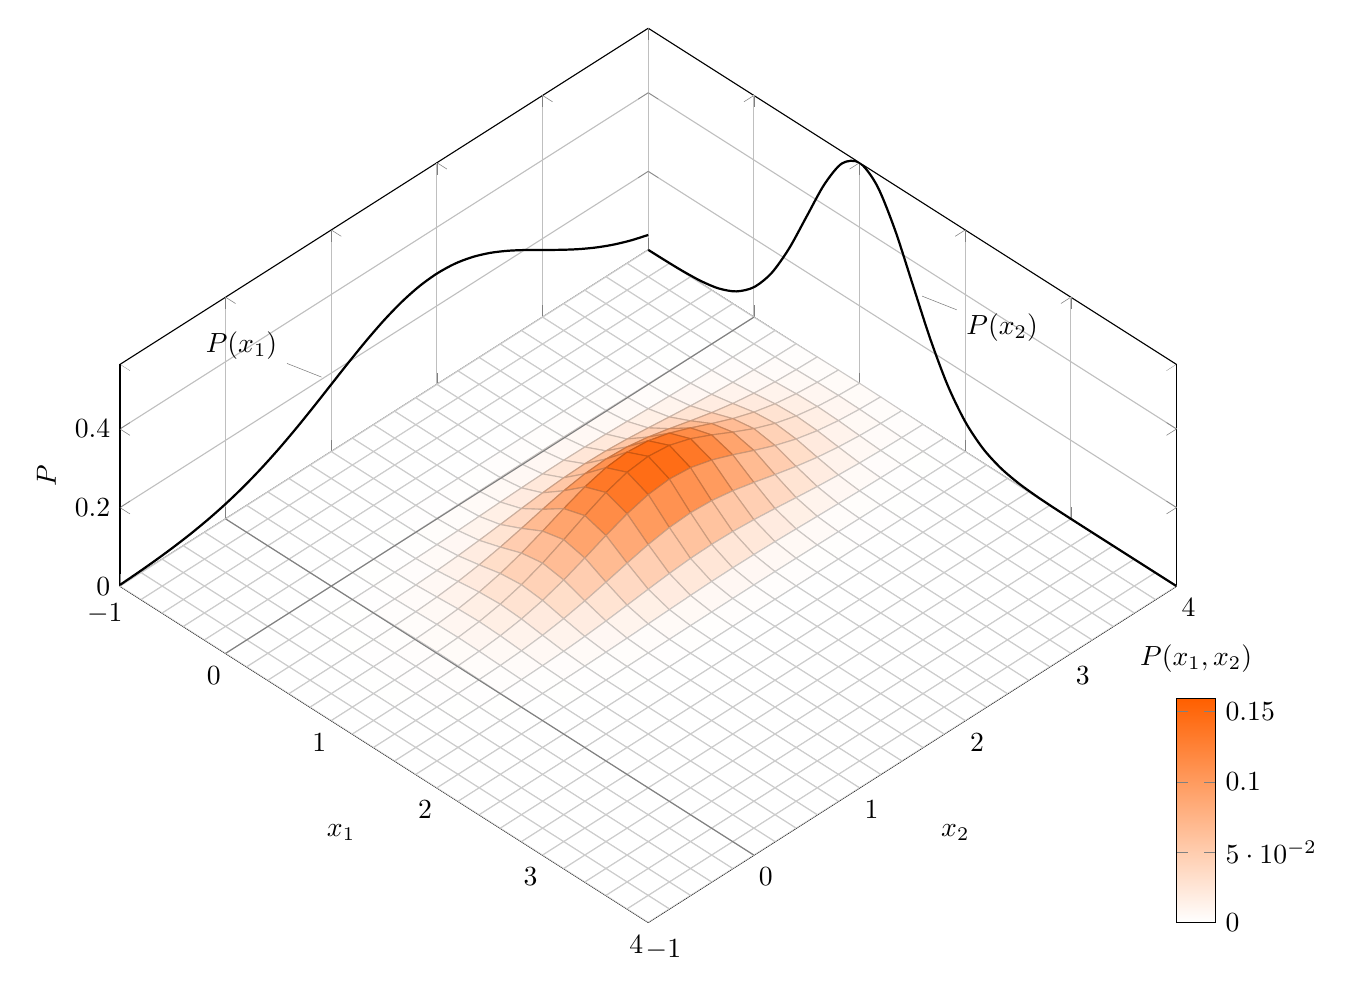
\begin{tikzpicture}[
    declare function = {mu1=1;},
    declare function = {mu2=2;},
    declare function = {sigma1=0.5;},
    declare function = {sigma2=1;},
    declare function = {normal(\m,\s)=1/(2*\s*sqrt(pi))*exp(-(x-\m)^2/(2*\s^2));},
    declare function = {bivar(\ma,\sa,\mb,\sb)=
      1/(2*pi*\sa*\sb) * exp(-((x-\ma)^2/\sa^2 + (y-\mb)^2/\sb^2))/2;}]
    \begin{axis}[
      colormap name  = whitered,
      width          = 15cm,
      view           = {45}{65},
      enlargelimits  = false,
      grid           = major,
      domain         = -1:4,
      y domain       = -1:4,
      samples        = 26,
      xlabel         = $x_1$,
      ylabel         = $x_2$,
      zlabel         = {$P$},
      colorbar,
      colorbar style = {
        at     = {(1,0)},
        anchor = south west,
        height = 0.25*\pgfkeysvalueof{/pgfplots/parent axis height},
        title  = {$P(x_1,x_2)$}
      }
    ]
      \addplot3 [surf] {bivar(mu1,sigma1,mu2,sigma2)};
      \addplot3 [domain=-1:4,samples=31, samples y=0, thick, smooth]
        (x,4,{normal(mu1,sigma1)});
      \addplot3 [domain=-1:4,samples=31, samples y=0, thick, smooth]
        (-1,x,{normal(mu2,sigma2)});
  
      \draw [black!50] (axis cs:-1,0,0) -- (axis cs:4,0,0);
      \draw [black!50] (axis cs:0,-1,0) -- (axis cs:0,4,0);
  
      \node at (axis cs:-1,1,0.18) [pin=165:$P(x_1)$] {};
      \node at (axis cs:1.5,4,0.32) [pin=-15:$P(x_2)$] {};
    \end{axis}
  \end{tikzpicture}

\section{Reference}
\bibliography{Distributedlaggedmodel.bib}
\end{document}

